\documentclass[journal]{IEEEtran}

% *** FLOAT PACKAGES ***
%
%\usepackage{fixltx2e}
% fixltx2e, the successor to the earlier fix2col.sty, was written by
% Frank Mittelbach and David Carlisle. This package corrects a few problems
% in the LaTeX2e kernel, the most notable of which is that in current
% LaTeX2e releases, the ordering of single and double column floats is not
% guaranteed to be preserved. Thus, an unpatched LaTeX2e can allow a
% single column figure to be placed prior to an earlier double column
% figure.
% Be aware that LaTeX2e kernels dated 2015 and later have fixltx2e.sty's
% corrections already built into the system in which case a warning will
% be issued if an attempt is made to load fixltx2e.sty as it is no longer
% needed.
% The latest version and documentation can be found at:
% http://www.ctan.org/pkg/fixltx2e


%\usepackage{stfloats}
% stfloats.sty was written by Sigitas Tolusis. This package gives LaTeX2e
% the ability to do double column floats at the bottom of the page as well
% as the top. (e.g., "\begin{figure*}[!b]" is not normally possible in
% LaTeX2e). It also provides a command:
%\fnbelowfloat
% to enable the placement of footnotes below bottom floats (the standard
% LaTeX2e kernel puts them above bottom floats). This is an invasive package
% which rewrites many portions of the LaTeX2e float routines. It may not work
% with other packages that modify the LaTeX2e float routines. The latest
% version and documentation can be obtained at:
% http://www.ctan.org/pkg/stfloats
% Do not use the stfloats baselinefloat ability as the IEEE does not allow
% \baselineskip to stretch. Authors submitting work to the IEEE should note
% that the IEEE rarely uses double column equations and that authors should try
% to avoid such use. Do not be tempted to use the cuted.sty or midfloat.sty
% packages (also by Sigitas Tolusis) as the IEEE does not format its papers in
% such ways.
% Do not attempt to use stfloats with fixltx2e as they are incompatible.
% Instead, use Morten Hogholm'a dblfloatfix which combines the features
% of both fixltx2e and stfloats:
%
% \usepackage{dblfloatfix}
% The latest version can be found at:
% http://www.ctan.org/pkg/dblfloatfix

% Citation package
\usepackage{cite}

% graphic package
\ifCLASSINFOpdf
  \usepackage[pdftex]{graphicx}
  \DeclareGraphicsExtensions{.pdf,.jpeg,.png}
\else
  % \usepackage[dvips]{graphicx}
  % \DeclareGraphicsExtensions{.eps}
\fi

% math package
\usepackage{amsmath,amsfonts,amssymb,amscd,amsthm,xspace}
\usepackage{array}

% subfigure package
\ifCLASSOPTIONcompsoc
  \usepackage[caption=false,font=footnotesize,labelfont=sf,textfont=sf]{subfig}
\else
  \usepackage[caption=false,font=footnotesize]{subfig}
\fi

% tikz for graphs
\usepackage{tikz}
\usetikzlibrary{arrows,shapes,snakes,automata,backgrounds,petri}

% other necesssary packages
\usepackage{multirow}
\usepackage{times}

% correct bad hyphenation here
\hyphenation{spe-ci-fi-cal-ly re-gu-la-ted ge-ne-ra-li-sa-ti-on fun-ding dif-fe-rent pa-ra-me-ter a-ve-ra-ging ha-ving bia-ses va-lu-es in-fe-ren-ce theo-rem pro-ba-bi-li-ty ap-pro-xi-ma-ti-on ma-xi-mi-sing u-sing e-le-ments de-fi-ni-ti-on}

\begin{document}

\title{Partially Observable Count Estimation by an Autonomous Mobile Robot}
% \title{Spectral-POPP for Robot Exploration in Partially Observable Environments}

\author{Ferdian~Jovan, Milan Tomy Mariya, Jeremy Wyatt, Nick Hawes 
% \IEEEcompsocitemizethanks{\IEEEcompsocthanksitem F. Jovan is with the Department
% of Engineering Science, University of Oxford, Oxford, OX1~3PJ.\protect\\
% E-mail: ferdian.jovan@gmail.com 
% \IEEEcompsocthanksitem Jeremy Wyatt is with the Department of Computer Science, University of Birmingham, Birmingham, B15~2TT.
% \IEEEcompsocthanksitem Nick Hawes is with Oxford Robotics Institute, Oxford, OX2~6NN. 
% }% <-this % stops an unwanted space
% \thanks{Manuscript received April 19, 2005; revised August 26, 2015.}
}

% The paper headers
\markboth{IEEE TRANSACTIONS ON ROBOTICS, VOL. XX, NO. X, MONTH YEAR}%
{Shell \MakeLowercase{\textit{et al.}}: Bare Demo of IEEEtran.cls for IEEE Journals}

% make the title area
\maketitle

\begin{abstract}
    The Poisson assumption is a popular choice when data arises in the form of counts. In many applications such as in mobile robotics, such counts are prone to a systematic error due to unreliable sensor algorithms and the data set that result can not be trusted. Only limited works have been done on the Poisson model when a full observability of the data is in question. We present practical Bayesian estimators in this paper for a partially observable Poisson process (POPP). Variations of these processes are presented, in which (i) sensors are uncorrelated, (ii) sensors are correlated, (iii) the unreliability of the observation model, when built from data, is accounted for. The actual posterior distributions are estimated via two tractable approximations, which we combined in a switching filter. The filter enables efficient and accurate estimation of the posterior. A detailed empirical analysis is performed on both simulated and real-world data, and an application of the resulting posterior to drive exploration of a mobile robot with unreliable sensors is presented. 
\end{abstract}

\begin{IEEEkeywords}
Poisson processes, partial observability, misclassified counts, robot exploration
\end{IEEEkeywords}


\IEEEpeerreviewmaketitle

\section{Introduction}
\label{sec:introduction}

In recent years, autonomous mobile robots have started to come to assist humans with simple daily tasks in our homes and offices \cite{hawes2016strands}. As the robot is expected to work in dynamic environments, any behaviour model for the robot to adapt with humans is typically learnt over time from observations \cite{coppola2016learning}. Where these observations are made using sensor data, both humans and all the currently robotic sensory systems have some level of unreliability. This means collected data-sets that make up the observations typically contain systematic errors that lead to bias in the statistical estimate produced by the sensors. In this paper, we address the unreliability problem of sensors counting events by formulating a \textit{partially observable Poisson process} (POPP). As we may require it do so for when multiple sensors are involved in which one sensor may (or may not) correlate to one another, we extend the POPP model with several variations. A standard fully observable Poisson process (FOPP) is introduced to distinct the POPP and its derivatives from it.

Several practical contributions are made. First, a set of inference methods for a Poisson process which take into account the unreliability of either single or multiple sensory systems used to count events is addressed. Two tractable approximations to the posterior of such Poisson processes, which are combined into a switching filter, are presented to cope with the absence of a conjugate density. One (the \textit{Gamma filter}) is fast, but prone to drift from the true posterior in certain circumstances. The second (the \textit{histogram filter}) is slower but avoids drifts. Variations of these processes are introduced. First is the correlated POPP (C-POPP) to deal with sensors that are correlated to one another. The second variation is the POPP-Beta which deals with the unreliability of the observation model. We also combine the C-POPP and the POPP-Beta in the POPP-Dirichlet model that is able to deal with correlated sensors and the unreliability of the observation model. We demonstrate the properties of the POPP, its variations, and its filters by numerical simulations and real-world datasets.

Finally, we show the benefit of the POPP model, and its variation on a robot exploration task performed by a mobile robot. The resulting posterior of the POPP and its derivative is used to drive exporation by a mobile robot for a series of two week deployment. Robot exploration rises from the fact that any mobile robot needs to observe human activities/behaviour in order to learn and adapt in its human-populated environment. As the robot has a limit to its operational life, one would therefore like it to optimise the time it takes to build its models. We contrast this with an exploration method based on the FOPP model. We show that the exploration method involving corrections to systematic errors doubles the number of human encounters the robot experiences. 

% We show variations of the exploration methods based on optimistic predictions from the resulting posteriors of the first contribution. 
% BELUM BERES INI
% The second contribution is the variation of exploration methods for a mobile robot based on optimistic predictions from the resulting posteriors of the first contribution. As any mobile robot in human-populated environment needs to learn human behaviour/activity, it must first explore where activities are likely to happened and observe them. One would like the robot to observe a sufficient amount of human activity, so as to learn the specific kinds of activity models. However, as a mobile robot can only be in one place at one time, its observations are spatially restricted. Moreover, the robot has a limit to its operational life. We would therefore like it to optimise the time it takes to build its models. This introduces an exploration-exploitation trade-off problem \cite{wyatt1998exploration, 1413255, AUDIBERT20091876}, i.e. should the robot visit a familiar place, where it will probably observe two activities, or go to a new place, where it might observe many more but might see nothing? 

% is expected to work around and/or with humans, modelling human activities becomes a necessity. In any scenario where a robot learns about human activities, it must first explore where activities are likely to happened and observe them. 
% 
% One would like the robot to observe a sufficient amount of human activity, so as to learn the specific kinds of activity models. However, as a mobile robot can only be in one place at one time, its observations are spatially restricted. Moreover, the robot has a limit to its operational life. We would therefore like it to optimise the time it takes to build its models. This introduces an exploration-exploitation trade-off problem \cite{wyatt1998exploration, 1413255, AUDIBERT20091876}, i.e. should the robot visit a familiar place, where it will probably observe two activities, or go to a new place, where it might observe many more but might see nothing?
% 
% Another important restriction in mobile robotics is that robot sensors are unreliable. Any solution must take into account the unreliability of sensors. We may also require that it do so for when multiple sensors are involved. This means that collected data which are used for learning typically contain systematic errors that lead to bias in the statistical estimates produced by the event detection processes.

% To allow the robot to observe a sufficient amount of human activity, so as to learn the specific kinds of activity models, putting an exploration to places with high number of activities becomes a mandatory action. There are several reasons behind this. First, a mobile robot can only be in one place at one time, so its observations are spatially restricted.   
% 
% The problem of this thesis can be loosely formulated as how to predict where many people are most likely to be and to go and observe them. Specifically, it requires the robot to go to where the aggregate level of human activity is highest. In addition, this thesis chooses to tackle the problem for the case where the robot runs for an extended period of time such days, or even weeks as it builds its models.
% A key challenge is for the robot to be able to recognise and react adequately to dynamic changes that happen in human-centered environments, especially when the changes are the result of human behaviour. The learning process for an autonomous mobile robot to adapt to its environment takes a big portion of its lifetime and it needs to deal with the huge volume of experiences accessible to it as it runs for longer periods of time. One advantage of all these is that these experiences contain potentially useful information that can help the robot to eventually adapt to its environment.

% Taken together, the challenges and benefits faced by an autonomous mobile robot motivate this thesis to create long-term understanding of temporal dynamics of human activities, along with the ability to exploit this understanding for a better adaptation of an autonomous mobile robot. The robot is expected to demonstrate its ability to predict future activities based on its statistical model. It is also expected to be able to detect anomalies as sequences of very low likelihood data.



%!TEX root = ../bare_jrnl.tex

\section{Fully Observable Poisson Process}
\label{sec:preliminaries}

A \emph{fully observable} Poisson process (FOPP) models the distribution of $N(t)$, the number of events appearing in time interval $[0, t)$, parameterised by an \textit{arrival rate}, $\lambda$:
\begin{equation}
    \label{eq:pmf_poisson}
	Poi(N(t) = c \mid \lambda) = \frac{e ^{-\lambda} \lambda ^{c}}{c!}
\end{equation}
We use $N(t) = c_i$ to refer to a count recorded during the $i$-th observation of the process.
Given a Gamma density
\begin{equation}
    \label{eq:pdf_gamma}
    \begin{tabular}{rcl}
        $Gam(\lambda \mid \alpha, \beta)$ & = & $\displaystyle\frac{\beta ^{\alpha}}{\Gamma (\alpha)} \lambda ^{\alpha - 1} e^{-\beta \lambda}$ \\ [1ex]
    \end{tabular}
\end{equation}
as a prior distribution over the parameter $\lambda$, where $\alpha, \beta$ are the shape and the rate parameters, the posterior over $\lambda$ for a FOPP can be  calculated via Bayesian inference with
\begin{equation}
    \label{eq:posterior_fopp}
    \begin{array}{lll}
        P(\lambda \mid c_1, \ldots, c_n) & \varpropto Poi(c_1, \ldots, c_n \mid \lambda) ~ Gam(\lambda \mid \alpha, \beta) \\
         & = Gam \Bigg(\lambda \Bigm| \displaystyle\sum_{i=1}^{n} \alpha + c_i, \beta + n \Bigg)
    \end{array}
\end{equation}
This adds the sample counts $\sum_{i=1}^{n} c_i$ to the hyper-parameter $\alpha$ of the gamma prior, and adds the number of observations $n$ to the hyper-parameter $\beta$ of the gamma prior.

The FOPP model requires a single reliable sensor. With an unreliable sensor, FOPP inferences will be incorrect.
\section{Related Work}
\label{sec:related}

There are some existing works which address statistical models where the observation data are not fully observable. In some literature, this effect is regarded as misclassified counts. Misclassification happens when there are false positive counts or false negative counts (or possibly both). False positive counts, which can also be called the overcount, are when the count includes events other than those of interest. Whereas false negative counts, which can also be called the undercount, are when some of the events of interest are missed or omitted. Early work on this involving count data dealt with the undercount (or under-reporting) problem as this is quite a common problem. Whittemore and Gong estimated cervical cancer rates by taking into account false negative data \cite{whittemore1991}. Winkelmann and Zimmermann introduced a combination of a Poisson regression model with a logit model for under-reporting, yielding the Poisson-Logistic (Pogit) model \cite{winkelmann1993poisson}. They applied this to model the number of days employees were absent from a workplace. Dvorzak and Wagner borrowed the Pogit model and incorporated a small set of validation data, which is assumed available, to provide information about the true counts \cite{dvorzak2016}. A Bayesian analysis of the Poisson-Logistic model was performed and Bayesian variable selection was incorporated to identify regressors with a non-zero effect and also to restrict parameters of the Poisson-Logistic model.

Fewer worked on the Poisson model in the case when the count data may either be undercounting or overcounting \cite{sposto1992, bratcher2002, bratcher2004, stamey2005}. Sposto et al. estimated both cancer and non-cancer death rates, assuming false negatives are possible on both sides of these counts \cite{sposto1992}. The approach used by them followed the frequentist framework. Bratcher and Stamey, in \cite{bratcher2002}, used a Bayesian method to estimate Poisson rates in the presence of both undercounts and overcounts borrowing the double sampling technique introduced in \cite{Tenenbein1970}. They then extended their work to a fully Bayesian method for interval prediction of the unobservable actual count in future samples, given a current double sample \cite{bratcher2004}. Stamey and Young \cite{stamey2005} managed to obtained closed-form expressions for maximum likelihood estimators of the false negative rate, the false positive rate, and the Poisson rate for the model proposed in \cite{bratcher2002}. The estimators are straightforward to calculate and to interpret in terms of evaluating the effectiveness of using unreliable counts.

Our work is similar to the work in \cite{bratcher2002} to accurately estimate the parameter of a single Poisson process. They utilised the double sampling technique to obtain the true count together with false positive count and false negative count. The Poisson rate is estimated via an MCMC approximation due to no-closed form and expensive calculation of the posterior distribution of $\lambda$. Our work differs from theirs in that they are interested in estimation of a single Poisson process where the estimation is based on two counters with one always being a perfect counter. Here, we consider multiple unreliable counters, which may have correlations to one another, applied to estimating the parameter of a single Poisson process. To tackle the non-trivial density of the posterior, three precise and tractable Bayesian estimators are proposed. 

Our work is actually an extension to the work in \cite{jovan18a} in accurately estimating the parameter of a single Poisson process to improve its prediction accuracy. We present three further extensions of the original model presented in \cite{jovan18a} and their applications to exploit the temporal dynamics in the aggregate level of human activities for better robot exploration.

% involved binomial and multinomial models \cite{Bross1954,Chen1979,Hochberg1977,Tenenbein1970,Viana1993}. The first technique which was recorded to handle misclassification was double sampling. It was first introduced by Tenenbein to correct for misclassification of binomial data and obtain a maximum likelihood estimate \cite{Tenenbein1970}. The double sampling approach utilizes two search techniques to retrieve relevant information: an expensive classification technique to obtain the true count along with the false positive count and false negative count from typically a small sample set, and a less-expensive classification technique only for error-prone counts on a larger sample set. The results of both counts are then combined to obtain estimators for the Poisson rate $\lambda$, and also for the misclassification parameters. The work of Tenenbein was then extended by Chen \cite{Chen1979} and Hochberg \cite{Hochberg1977} to correct misclassified counts in categorical and multinomial models to obtain maximum likelihood estimates. The double sampling technique was also extended to incorporate prior distributions in the binomial model and the posterior was obtained via Bayesian estimation \cite{Viana1993}. Bekele extended the work of \cite{Viana1993} by introducing a weighted prior scheme and allowing for several sources of information, including expert opinions \cite{bekele1998binomial}.

% Different than the case of binomial and multinomial models, only a few studies are found working on the effect of partial observability of the data on the Poisson distribution. Many deal 

\section{The POP Process}
\label{sec:popp}

The partially observable Poisson process (POPP) is a counting process $N(t)$ with arrival rate $\lambda$ where the number of events that occurred up to time $t$ are obtained by unreliable (possibly multiple) counters. The definition brings a distinction between \emph{true count} (or simply \emph{count}), which refers to the number of events that actually happened, and the \emph{sensed count}, which refers to the count obtained by a counter (or sensor). Given that $c_i$ number of events happened (as the true count) over the interval $[0, t)$ during the $i$-th observation, and $m$ counters observed the events unreliably, thus the sensed count $s_{ji}$ is the count given by sensor $j$ in the $i$-th observation within the interval $[0, t)$ with $0 \leq j \leq m$. 

\begin{figure}[t!]
	\centering
	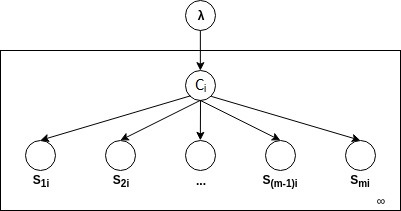
\includegraphics[width=0.5\textwidth]{./figures/gm_popp.jpg}
    \caption{Graphical representation of the partially observable Poisson process.}
	\label{fig:gm_popp}
\end{figure}

The graphical model, which is easily derived from the definition of the POPP, shows that the true count $c_i$ has become a latent variable which can only be inferred from the sensed count $\overrightarrow{s_i} = (s_{1i}, \ldots, s_{mi})$ where each $s_{ji}$ is a sensed count coming from sensor $j$. The posterior of $\lambda$ is then inferred from the posterior of $c_i$ after multiple samples $i = 1 \ldots n$.

A statistical inference to estimate the rate parameter $\lambda$ of the POPP model is done with a marginalisation over all possible true count value $c_i$ in a joint distribution between the posterior $P(\lambda ; c_i)$ and the posterior over $c_i$ given $\overrightarrow{s_i}$. The posterior of $\lambda$, given $n$ samples $\overrightarrow{s}=(\overrightarrow{s_1} \dots \overrightarrow{s_n})$, each consisting of $m$ sensors, is:
\begin{equation}
	\label{eq:marginal_occurrences}
	\begin{tabular}{r@{=}l}
		$P(\lambda ; \overrightarrow{s})$ &  $\displaystyle\sum_{c_1=0}^{\infty} \ldots \displaystyle\sum_{c_n=0}^{\infty} P(\lambda ; \overrightarrow{c}) ~ P(\overrightarrow{c} ; \overrightarrow{s})$ \\
	\end{tabular}
\end{equation}
\noindent where
\begin{equation*}
	\begin{tabular}{r@{ = }l}
		$P(\lambda ; \overrightarrow{c})$ & $Gam\Bigg(\lambda ; \displaystyle\sum_{i=1}^{n} c_i + \alpha, n + \beta \Bigg)$
	\end{tabular}
\end{equation*}
\noindent with $\overrightarrow{c} = (c_1, \ldots, c_n)$ for $1 \leq i \leq n$.

$P(\overrightarrow{c} ; \overrightarrow{s})$ is factored based on the assumption that each sensor is \textit{uncorrelated} to one another given the true count $c_i$. Consequently, the probability that the vector of true counts is $\overrightarrow{c}$, given $n$ samples of the vector of $m$ sensed counts $\overrightarrow{s_1}, \ldots, \overrightarrow{s_n}$, is

\begin{equation}
    \label{eq:occurrences_likelihood}
    \begin{tabular}{r@{ $\varpropto$ }l}
        $P(\overrightarrow{c} ; \overrightarrow{s_1}, \ldots, \overrightarrow{s_n})$ & $P(\overrightarrow{s_1}, \ldots, \overrightarrow{s_n} ; \overrightarrow{c}) ~ P(\overrightarrow{c})$ \\ [1ex]
        & $\displaystyle\prod_{i=1}^{n} P(\overrightarrow{s_i} ; c_i) ~ P(c_i)$ \\ [2ex]
        & $\displaystyle\prod_{i=1}^{n} \displaystyle\prod_{j=1}^{m} P(s_{ji} ; c_i) ~ P(c_i ; \overrightarrow{c_{-1}})$
    \end{tabular}
\end{equation}

\noindent where $\overrightarrow{c_{-1}} = c_{i-1}, \ldots, c_1$.

$P(c_i ; \overrightarrow{c_{-1}})$ and $P(s_{ji} ; c_i)$ are defined to complete Eqn. \ref{eq:occurrences_likelihood}. $P(c_i ; \overrightarrow{c_{-1}})$ is calculated in the form of a negative binomial distribution

\begin{equation}
	\label{eq:unconditional_xi}
	\begin{tabular}{r@{=}l}
		$P(c_i ; \overrightarrow{c_{-1}})$ & $\displaystyle\int_{\lambda=0}^{\infty} P(c_i ; \lambda) ~ P(\lambda ; \overrightarrow{c_{-1}}) ~d\lambda$ \\ [2ex]
		& $\displaystyle\int_{\lambda=0}^{\infty} Poi(c_i ; \lambda) ~ Gam(\lambda ; \alpha, \beta) ~d\lambda$ \\ [2ex]
		& $NB\Bigg(c_i ; \alpha, \displaystyle\frac{\beta}{\beta + 1}\Bigg)$.
	\end{tabular}
\end{equation}

The Poisson limit theorem states that the Poisson distribution may be used as an approximation to the binomial distribution \cite{papoulis2002probability}. Using this theorem as the foundation, an arbitrarily close approximation to the probability $P(s_{ji} ; c_i)$ is defined by assuming there exists a small enough finite subinterval of length $\delta$ for which the probability of more than one event occurring is less than some small value $ \epsilon$. With this assumption, interval $[0, t)$ is splitted into $l$ smaller subintervals $I_1, \ldots, I_l$ of equal size, with the condition that $l > \lambda$ (the condition is crucial since we focus on very small portions of the interval). Consequently, the whole interval $[0, t) = I_1, \ldots, I_l$ becomes a series of Bernoulli trials, where the $k^{th}$ trial corresponds to whether (1) an event $e_k$ happens with probability $\lambda / l$ and (2) a sensor $j$ captures the event $e_k$ as the detection $d_k$ at the subinterval $I_k$.

$P(s_{ji} ; c_i)$ is defined as the aggregate of the true positives $tp_{ji}$ in $c_i$ subintervals, and the false positives $fp_{ji}$ in $l-c_i$ subintervals. The probability of a \textit{true positive detection} (TP) for sensor $j$ in a subinterval is $tpr_j = P_j(d = 1 ; e=1)$, and the probability of a \textit{false positive detection} (FP) is $fpr_j = P_j(d = 1 ; e=0)$. Thus $P(s_{ji} ; c_i)$ is defined as a sum of two binomial distributions $B(r ; n,\pi)$, where the aggregate is constrained to be $s_{ji}$: 

\begin{equation}
	\label{eq:joint_binomial_distribution}
    P(s_{ji} ; c_i) \! = \! \! \! \displaystyle\sum_{\textrm{tp}_{ji} = 0}^{c_{i}} \! \! B\Big(\textrm{tp}_{ji} ; c_i, \textrm{tpr}_j\Big) B\Big(\textrm{fp}_{ji} ; \Delta c_i, \textrm{fpr}_j \Big)
\end{equation}
\noindent where $s_{ji} = \textrm{tp}_{ji} + \textrm{fp}_{ji}$, $\textrm{tpr}_j = P_j(d=1 ; e=1)$, $\textrm{fpr}_j = P_j(d=1 ; e=0)$, and $\Delta c_i = (l - c_i)$.

Eqn.~\ref{eq:marginal_occurrences} shows the difficulty of belief state estimation in the POPP model since there is no conjugate density accomodating an analytical solution for the posterior over $\lambda$. Each sensed count sample $\overrightarrow{s_i}$ used to update the posterior of $\lambda$ adds a factor of countably infinite number of elements. The resulting posterior is a sum of countably infinite sums. One can place an upper bound $l$ on the maximum value of each $c_i$, but it still makes the number of elements in the posterior grow by a factor $l$ with every sensed count $\overrightarrow{s_i}$.  

With this difficulty noted, Jovan et al., proposed three efficient estimators, each of which offers an approximation to the true posterior $P(\lambda ; \overrightarrow{s})$. A more detailed presentation of these estimators is given in \cite{jovan18a}.

\section{The POPP Extensions}
\label{sec:popp_extensions}

Jovan et al., have shown that the POPP model is able to efficiently corrects miscounts made by multiple unreliable counting devices observing a single Poisson process \cite{jovan18a} . However, it was mentioned that the model is limited by two assumptions:
\begin{enumerate}
    \item the degree of the unreliability of a sensor is precisely known, and
    \item counter failures are conditionally independent from one to another given the true count. 
\end{enumerate}
In this work, we propose three gradual extensions to the POPP model to tackle the aforementioned assumptions. The first extension (POPP-Beta) is built on top of the POPP model to tackle the first assumption. The second extension (C-POPP) modifies the POPP model to tackle the second assumption. The third extension (POPP-Dirichlet) is built on top of the C-POPP model to tackle both assumptions together. 

\subsection{The C-POPP}

\subsection{The POPP-Beta}

\subsection{The POPP-Dirichlet}

\section{Conclusion}
\label{sec:conclusion}

This work has been concerned with developing practical estimators for count data collected by an autonomous mobile robot, with unreliable perception algorithms. These count data represent the level of human activity in particular locations. This work extends the work in \cite{jovan18a} with several contributions:

\begin{itemize} 
    % \item A set of inference methods for the partially observable Poisson process (POPP) has been formulated. The POPP is a Poisson process which takes into account the unreliability of the sensors that count events. Unlike Bayesian estimation for a fully observable Poisson process (FOPP), obtaining the posterior is non-trivial, since there is no conjugate density for a POPP and the posterior has a number of elements that grow exponentially in the number of observed intervals. Two simple, tractable, approximations have been presented. These two approximations are combined in a switching filter, which enables efficient and accurate estimation of the posterior. A simulation study shows that these POPP filters correct the over- and under-counts produced by sensors.  
    \item Variations of the POPP filter are presented. The POPP-Beta filter extends the POPP filter in which the unreliability of the observation model is accounted for when estimations are built. The N-POPP filter extends the POPP filter by modelling the case when sensors are uncorrelated. The POPP-Dirichlet combines the POPP-Beta filter and the N-POPP filter to have the benefits of each correction. A simulation and observations taken by a robot, on a series of long deployments, show that each extension provides progressively more accurate estimates than the POPP filter.  
    \item Both posteriors from the Spectral-FOPP and two Spectral-POPP processes are used to drive exploration by a mobile robot for a series of two week deployments. An upper bound interval exploration method was used to solve the exploration-exploitation problem. After labelling by humans, this resulted in a labelled data set of six weeks of human activity levels. A simulated study has shown that the Spectral-FOPP and the Spectral-POPP filter improve on-point observation time significantly if strong periodic patterns underlying the human activities are present. 
\end{itemize}
        
        % Finally, the various POPP filters are compared to one another and to a FOPP estimator on this data set.

% which capture the regular structures of dynamic behaviours, especially humans,    
% 
% 
% Hence, any learning algorithm requires practical estimation which capture temporal structures of human activities.   
% 
% The adaptation requires practical estimation which capture the structure 
% 
% The robot will be able to demonstrate that it can recognise activities at various
% temporal scales, and infer or predict future activities based on its temporal model (e.g. it
% might go to the lounge because it has just seen the residents finishing their lunch). It
% will also be able to detect anomalies as sequences of very low likelihood data.
% 
% The robot only observes a limited portion of the space at any time, and so must actively plan to go to places to observe events.
% 
% learns dynamic behaviours of its surrounding while patroling around perimeters of a large area. 
% 
% Human activities follow predictable, repeating patterns that generate corresponding
% changes in space.
% 
% Our
% work will allow a robot to create a map of a building and its contents: not just walls but people,
% furniture and objects, all in a unified spatial-temporal representation that will allow a robot to
% respond robustly to the dynamics of its environment. In order to reason about the structure
% and purpose of these dynamics we will employ the spatial-temporal representations in support of
% activity recognition. This will allow the robot to detect, and exploit, patterns of human behaviour.
% 
% In our care scenario we will explore how a robot can support staff working with a small group of
% elderly patients in a nursing facility. The robot will learn about the patients’ regular activities. It
% will use this knowledge to perform support tasks for the care staff and serve as an early warning
% system when patients vary from regular behaviour (e.g. wandering the corridors at night, falling
% over). In our security scenario we will explore how a robot can act as a security guard, performing
% patrols to learn the typical spatial-temporal structures in a building and notifying a human guard
% of suspicious variations from these.

% \section{Limitations and Further Work}
% 
% Two basic statistical models: Spectral-FOPP and POPP  have been proposed and evaluated. The combination of these two is able to extract temporal dynamics in the aggregate level of human activities from unreliable sensors, along with the ability to exploit this understanding for better exploration by an autonomous mobile robot. However, the spectral-POPP model could still be improved in the following two ways:
% \begin{enumerate}
%     \item In Chapter \ref{chap:popp_independent}, The Gamma filter approximates a sum of Gamma distributions with a single Gamma distribution assuming that the sensor performs rather reliable. Instead of using a single Gamma distribution to approximate a sum of $m$ Gamma distributions, $n$ gamma distributions, where $n$ is much smaller than $m$, could be used to improve the accuracy of the approximation to the posterior. This would promise to be more accurate than a single gamma, but more efficient than a histogram filter. Thus, it might be faster than the switching filter.
% 
%     \item The spectral-Poisson model (Spectral-FOPP) in Chapter \ref{chap:spectral_poisson} is a statistical model which is able, and only able, to capture the periodic structure of count data. It indirectly assumes that there is an underlying pattern governing the evolution of the parameter $\lambda$ of a Poisson process. The spectral-Poisson might not be able to capture other non-periodic structures governing the parameter $\lambda$, such as trends. 
% 
%         A Gaussian process modulated Poisson process might provide a better model for different structures which govern $\lambda$ overtime. Work from \cite{lloyd2015variational} presents a fully variational Bayesian inference scheme for continuous Gaussian-process modulated Poisson process. It provides a good estimators and is fast in estimating $\lambda$ of a Poisson process. An extension to this statistical model which embeds both trends and periodicity in the model might provide a solution to the limitations of Spectral-Poisson while being fully Bayesian. 
% \end{enumerate}

% Listing all limitations which have been mentioned in previous sections.
% Listing all further work which can extend this thesis.

\ifCLASSOPTIONcompsoc
  \section*{Acknowledgments}

\else
  \section*{Acknowledgment}
\fi

The research leading to these results has received funding from the European Union Seventh Framework Programme (FP7/2007-2013) under grant agreement No 600623, STRANDS.


% An example of a double column floating figure using two subfigures.
% (The subfig.sty package must be loaded for this to work.)
% The subfigure \label commands are set within each subfloat command,
% and the \label for the overall figure must come after \caption.
% \hfil is used as a separator to get equal spacing.
% Watch out that the combined width of all the subfigures on a 
% line do not exceed the text width or a line break will occur.
%
%\begin{figure*}[!t]
%\centering
%\subfloat[Case I]{\includegraphics[width=2.5in]{box}%
%\label{fig_first_case}}
%\hfil
%\subfloat[Case II]{\includegraphics[width=2.5in]{box}%
%\label{fig_second_case}}
%\caption{Simulation results for the network.}
%\label{fig_sim}
%\end{figure*}
%
% Note that often IEEE papers with subfigures do not employ subfigure
% captions (using the optional argument to \subfloat[]), but instead will
% reference/describe all of them (a), (b), etc., within the main caption.
% Be aware that for subfig.sty to generate the (a), (b), etc., subfigure
% labels, the optional argument to \subfloat must be present. If a
% subcaption is not desired, just leave its contents blank,
% e.g., \subfloat[].


% An example of a floating table. Note that, for IEEE style tables, the
% \caption command should come BEFORE the table and, given that table
% captions serve much like titles, are usually capitalized except for words
% such as a, an, and, as, at, but, by, for, in, nor, of, on, or, the, to
% and up, which are usually not capitalized unless they are the first or
% last word of the caption. Table text will default to \footnotesize as
% the IEEE normally uses this smaller font for tables.
% The \label must come after \caption as always.
%
%\begin{table}[!t]
%% increase table row spacing, adjust to taste
%\renewcommand{\arraystretch}{1.3}
% if using array.sty, it might be a good idea to tweak the value of
% \extrarowheight as needed to properly center the text within the cells
%\caption{An Example of a Table}
%\label{table_example}
%\centering
%% Some packages, such as MDW tools, offer better commands for making tables
%% than the plain LaTeX2e tabular which is used here.
%\begin{tabular}{|c||c|}
%\hline
%One & Two\\
%\hline
%Three & Four\\
%\hline
%\end{tabular}
%\end{table}

\ifCLASSOPTIONcaptionsoff
  \newpage
\fi

% trigger a \newpage just before the given reference
% number - used to balance the columns on the last page
% adjust value as needed - may need to be readjusted if
% the document is modified later
%\IEEEtriggeratref{8}
% The "triggered" command can be changed if desired:
%\IEEEtriggercmd{\enlargethispage{-5in}}

% REFERENCES
\bibliographystyle{IEEEtran}
\bibliography{biblio}

% biography section with photo
%\begin{IEEEbiography}[{\includegraphics[width=1in,height=1.25in,clip,keepaspectratio]{mshell}}]{Michael Shell}
% \begin{IEEEbiography}{Ferdian Jovan}
% Biography text here.
% \end{IEEEbiography}

% biography section without photo
\begin{IEEEbiographynophoto}{Ferdian Jovan}
Biography text here.
\end{IEEEbiographynophoto}

\begin{IEEEbiographynophoto}{Jeremy Wyatt}
Biography text here.
\end{IEEEbiographynophoto}

\begin{IEEEbiographynophoto}{Nick Hawes}
Biography text here.
\end{IEEEbiographynophoto}

% % insert where needed to balance the two columns on the last page with
% % biographies
% %\newpage
% 
% \begin{IEEEbiographynophoto}{Jane Doe}
% Biography text here.
% \end{IEEEbiographynophoto}

% You can push biographies down or up by placing
% a \vfill before or after them. The appropriate
% use of \vfill depends on what kind of text is
% on the last page and whether or not the columns
% are being equalized.

%\vfill

% Can be used to pull up biographies so that the bottom of the last one
% is flush with the other column.
%\enlargethispage{-5in}

\end{document}
